%!TEX root = ../Thesis.tex
\section*{Anhang}
\addcontentsline{toc}{section}{Anhang}
\fancyhead[R]{Anhang}

\anhangsverzeichnis

\anhang{Abbildungen}

\begin{figure}[hbt]
    \centering
    \begin{minipage}[t]{.95\textwidth}
        \caption[]{Layout-Datei und visuelle Ansicht in Android Studio}
        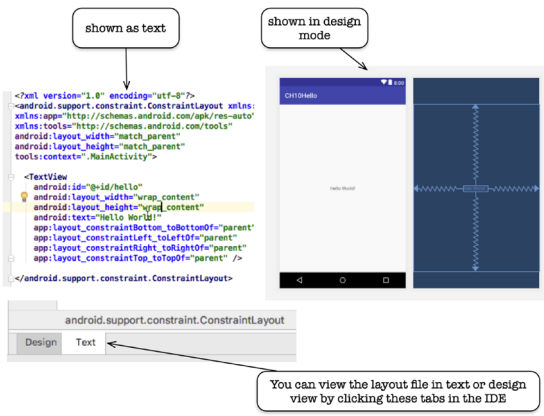
\includegraphics[width=1\textwidth]{img/Android_Studio_Layout_Editor.PNG}\\
        \source{\cite[36]{Hagos2020}}
        \label{fig:android_studio_layout_editor}
    \end{minipage}
\end{figure}

\begin{figure}[hbt]
    \centering
    \begin{minipage}[t]{.4\textwidth}
        \caption[]{Ordnerstruktur für manuelle Skalierung auf verschiedene Geräteklassen}
        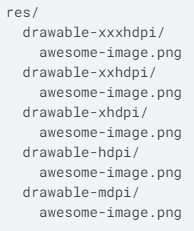
\includegraphics[width=1\textwidth]{img/DIP_Folder_Structure.PNG}\\
        \source{\cite{AndroidScreenDensities2020}}
        \label{fig:android_dip_folder_structure}
    \end{minipage}
\end{figure}

\begin{figure}[hbt]
    \centering
    \begin{minipage}[t]{.9\textwidth}
        \caption[]{Beispiel einer Karte}
        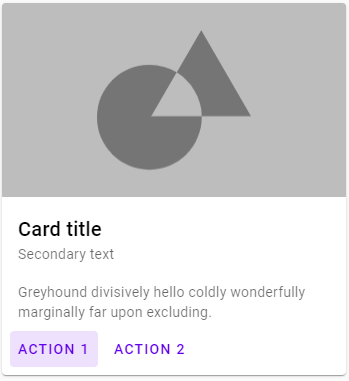
\includegraphics[width=1\textwidth]{img/Material_Card_Example.PNG}\\
        \source{\cite{MaterialCards2021}}
        \label{fig:material_card_example}
    \end{minipage}
\end{figure}

\begin{figure}[hbt]
    \centering
    \begin{minipage}[t]{.98\textwidth}
        \caption[]{Beispiel einer unteren Navigationsleiste}
        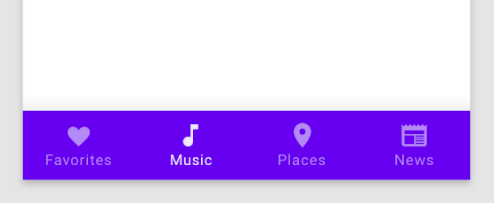
\includegraphics[width=1\textwidth]{img/Material_Bottom_Nav.PNG}\\
        \source{\cite{MaterialBottomNav2021}}
        \label{fig:material_bottom_nav_example}
    \end{minipage}
\end{figure}

\begin{figure}[hbt]
    \centering
    \begin{minipage}[t]{.98\textwidth}
        \caption[]{Beispiel einer oberen Leiste}
        
\includegraphics[width=1\textwidth]{img/Material_Top_Bar.PNG}\\
        \source{\cite{MaterialTopBar2021}}
        \label{fig:material_top_bar_example}
    \end{minipage}
\end{figure}

\begin{figure}[hbt]
    \centering
    \begin{minipage}[t]{.98\textwidth}
        \caption[]{Initiale Besprechung zum Projektstart}
        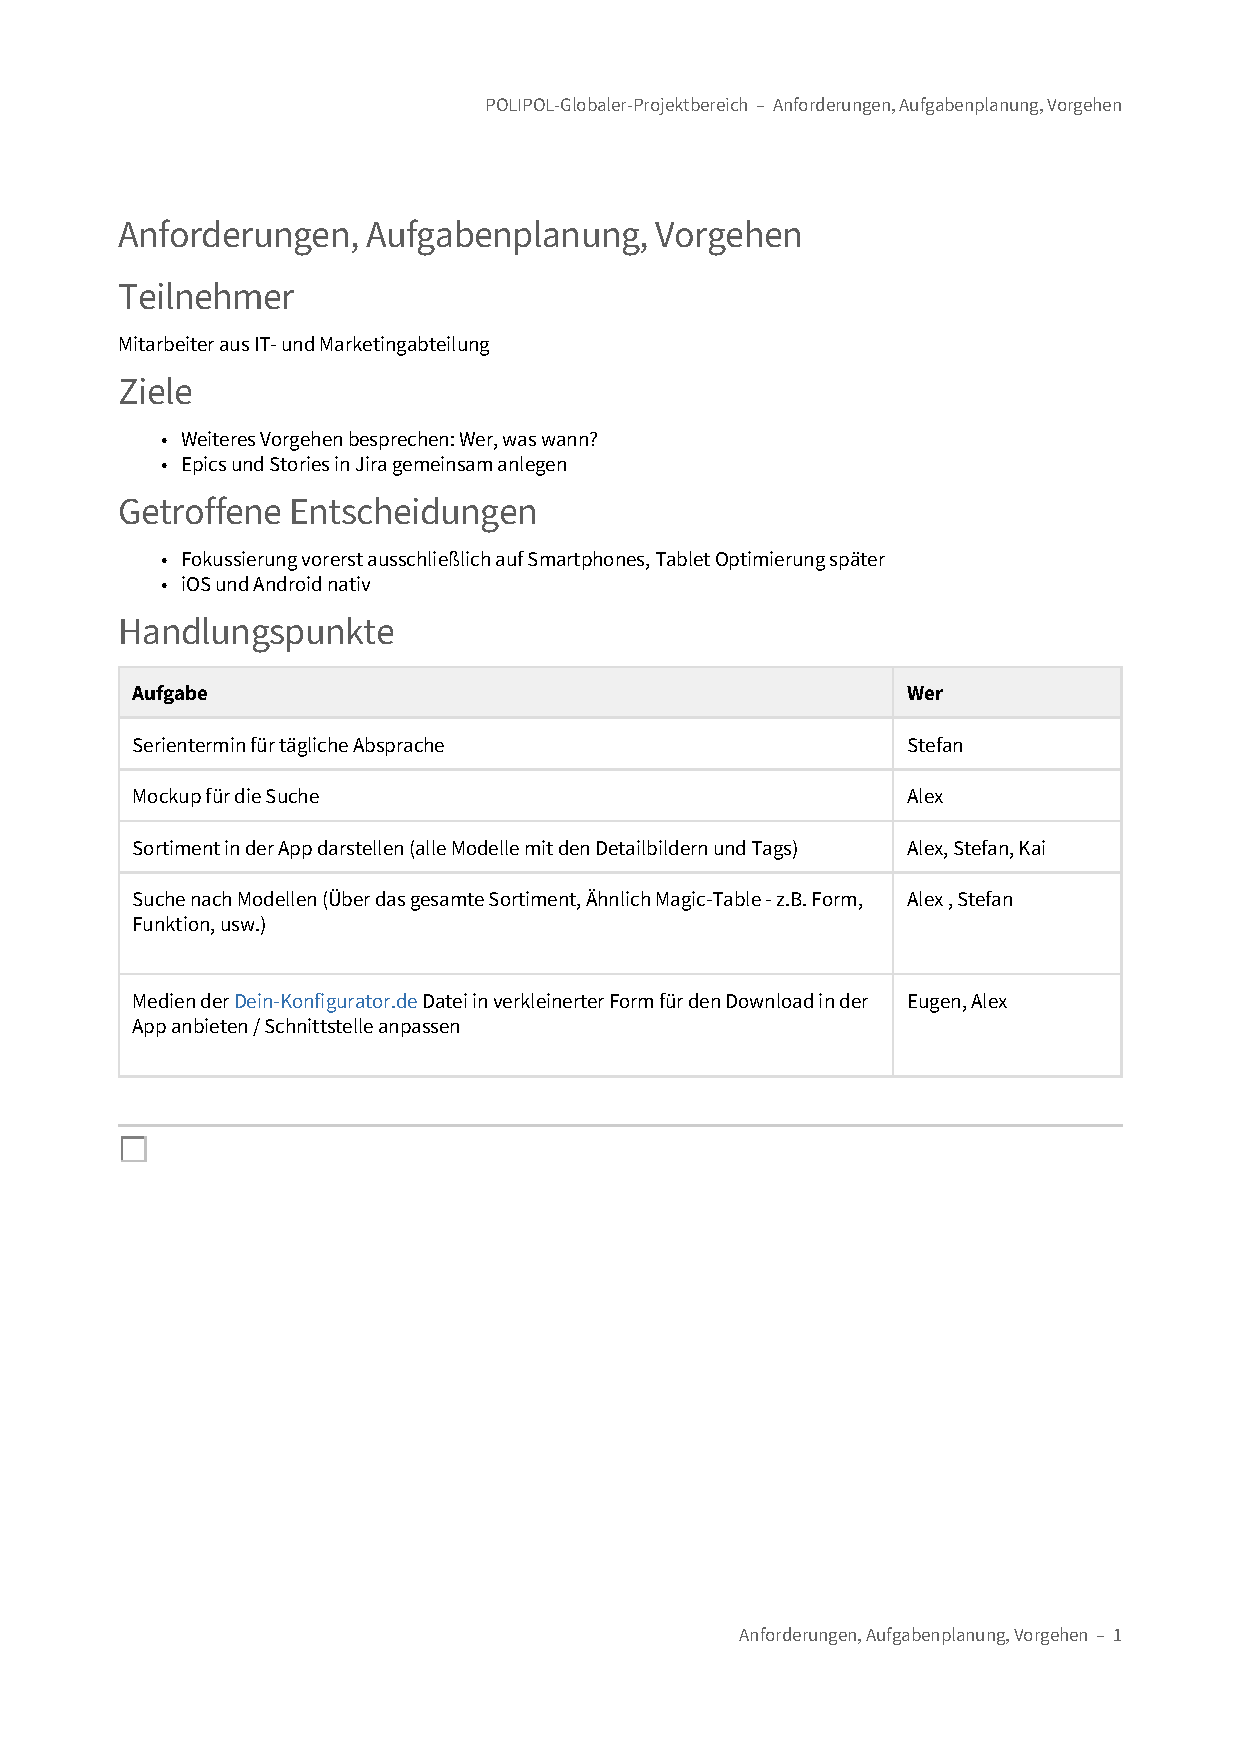
\includegraphics[width=1\textwidth]{img/Confluence_Anforderungsanalyse.pdf}\\
        \source{eigene Darstellung}
        \label{fig:initial_meeting}
    \end{minipage}
\end{figure}

\begin{figure}[!htb]
    \centering
    \begin{minipage}[t]{.4\textwidth}
        \caption{Typ 3AL}
        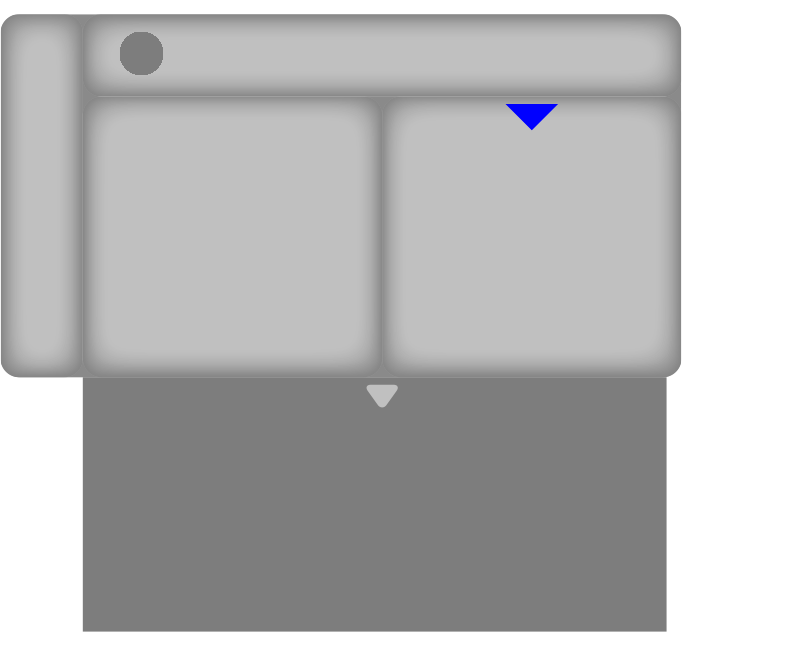
\includegraphics[width=1\textwidth]{img/Typ_3AL.png}\\
        \source{Polipol}
        \label{fig:type_plan_example_3al}
    \end{minipage}%
    \
    \begin{minipage}[t]{.4\textwidth}
        \caption{Kombinationen aus Typen bilden eine vollstände Garnitur}
        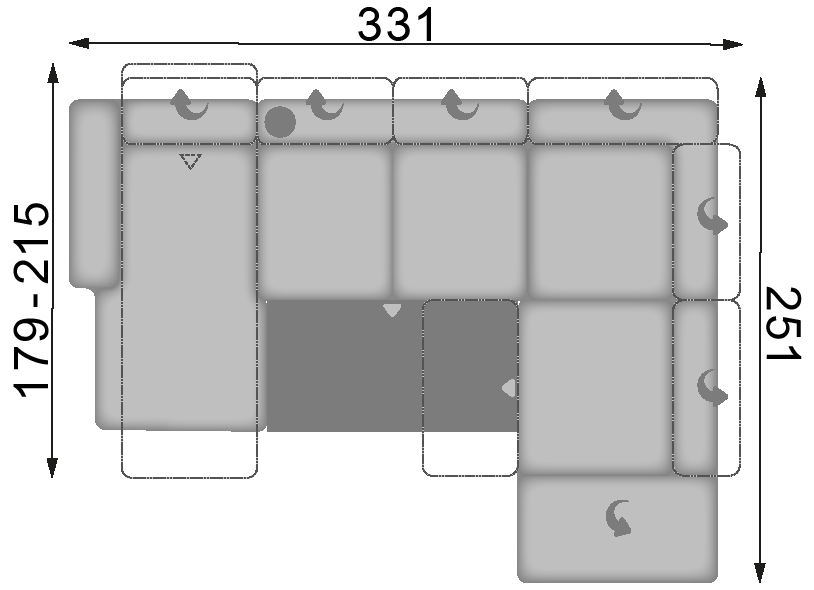
\includegraphics[width=1\textwidth]{img/Typen_Kombination.png}\\
        \source{Polipol}
        \label{fig:type_plan_example_combination}
    \end{minipage}
\end{figure}

\clearpage

\anhang{Tabellen}

\begin{table}[hbt]
    \centering
    \begin{minipage}[t]{1\textwidth} % Breite, z.B. 1\textwidth		
        \caption{User-Stories für Android} % Überschrift
        \begin{tabularx}{\columnwidth}{ |c|X| }
            \hline
            \textbf{Id} & \textbf{Beschreibung}                                                                                                                                                                              \\
            \hline
            IT-5373     & Als Verkäufer möchte ich alle Modelle im Sortiment, nach Sparten organisiert, mit Vorschaubildern und Namen betrachten können, um schnell einen Überblick über die verfügbaren Modelle zu bekommen \\
            \hline
            IT-5374     & Als Verkäufer möchte ich die Eigenschaften und unterstützten Funktionen zu einem Modell einsehen können, um den Kunden darüber informieren zu können
            \\
            \hline
            IT-5375     & Als Verkäufer möchte ich die Typen eines Modells einsehen können, um mögliche Kombinationen für einen Kunden erstellen zu können                                                                   \\
            \hline
            IT-5376     & Als Verkäufer möchte ich Bilder zu einem Modell einsehen können, um damit den Kunden etwas visuelles zeigen zu können                                                                              \\
            \hline
            IT-5378     & Als Verkäufer möchte ich ein Modell nach seinem Namen suchen können, um bekannte Modelle schnell zu finden                                                                                         \\
            \hline
            IT-5379     & Als Verkäufer möchte ich alle Modelle nach ihren Eigenschaften filtern können, um damit neue Modelle nach Kundenwünschen finden zu können                                                          \\
            \hline
            IT-5380     & Als Verkäufer möchte ich alle Modelle einer bestimmten Sparte nach ihren Eigenschaften filtern können, um meine Suche einzugrenzen                                                                 \\
            \hline
            IT-5381     & Als Verkäufer möchte ich alle Funktionen und ggf. Videos dazu einsehen können, damit ich die Endkunden über die Funktionsweise und Bedienung informieren kann                                      \\
            \hline
            IT-5382     & Als Verkäufer möchte ich alle verfügbaren Bezüge einsehen können, um den Kunden alle Möglichkeiten aufzeigen zu können
            \\
            \hline
            IT-5383     & Als Verkäufer möchte ich alle Farben zu einem Bezug einsehen können, um den Kunden über die Bezugsvarianten informieren zu können                                                                  \\
            \hline
            IT-5384     & Als Verkäufer möchte ich über Neuigkeiten (Messen, Schulungen) der Polipol-Gruppe informiert sein, um bei Bedarf an diesen teilzunehmen                                                            \\
            \hline
            IT-5385     & Als Verkäufer möchte ich die Webseite der Polipol-Gruppe aufrufen können, um mehr über den Möbelhersteller zu erfahren                                                                             \\
            \hline
        \end{tabularx}
        \source{eigene Darstellung}
        \label{tab:user_stories}
    \end{minipage}
\end{table}

\clearpage